\documentclass[compress]{beamer}
\usepackage{ifthen,verbatim}

\newcommand{\isnote}{}
\xdefinecolor{lightyellow}{rgb}{1.,1.,0.25}
\xdefinecolor{darkblue}{rgb}{0.1,0.1,0.7}

%% Uncomment this to get annotations
%% \def\notes{\addtocounter{page}{-1}
%%            \renewcommand{\isnote}{*}
%% 	   \beamertemplateshadingbackground{lightyellow}{white}
%%            \begin{frame}
%%            \frametitle{Notes for the previous page (page \insertpagenumber)}
%%            \itemize}
%% \def\endnotes{\enditemize
%% 	      \end{frame}
%%               \beamertemplateshadingbackground{white}{white}
%%               \renewcommand{\isnote}{}}

%% Uncomment this to not get annotations
\def\notes{\comment}
\def\endnotes{\endcomment}

\setbeamertemplate{navigation symbols}{}
\setbeamertemplate{headline}{\mbox{ } \hfill
\begin{minipage}{5.5 cm}
\vspace{-0.75 cm} \small
\end{minipage} \hfill
\begin{minipage}{4.5 cm}
\vspace{-0.75 cm} \small
\begin{flushright}
\ifthenelse{\equal{\insertpagenumber}{0}}{}{Jim Pivarski \hspace{0.2 cm} \insertpagenumber\isnote/\pageref{numpages}}
\end{flushright}
\end{minipage}\mbox{\hspace{0.2 cm}}\includegraphics[height=1 cm]{../cmslogo} \hspace{0.01 cm} \vspace{-1.05 cm}}

\begin{document}

%% \begin{notes}
%% \item This is the annotated version of my talk.
%% \item If you want the version that I am presenting, download the one
%% labeled ``slides'' on Indico (or just ignore these yellow pages).
%% \item The annotated version is provided for extra detail and a written
%% record of comments that I intend to make orally.
%% \item Yellow notes refer to the content on the {\it previous} page.
%% \item All other slides are identical for the two versions.
%% \end{notes}

\small

\begin{frame}
\frametitle{Geometry Models}
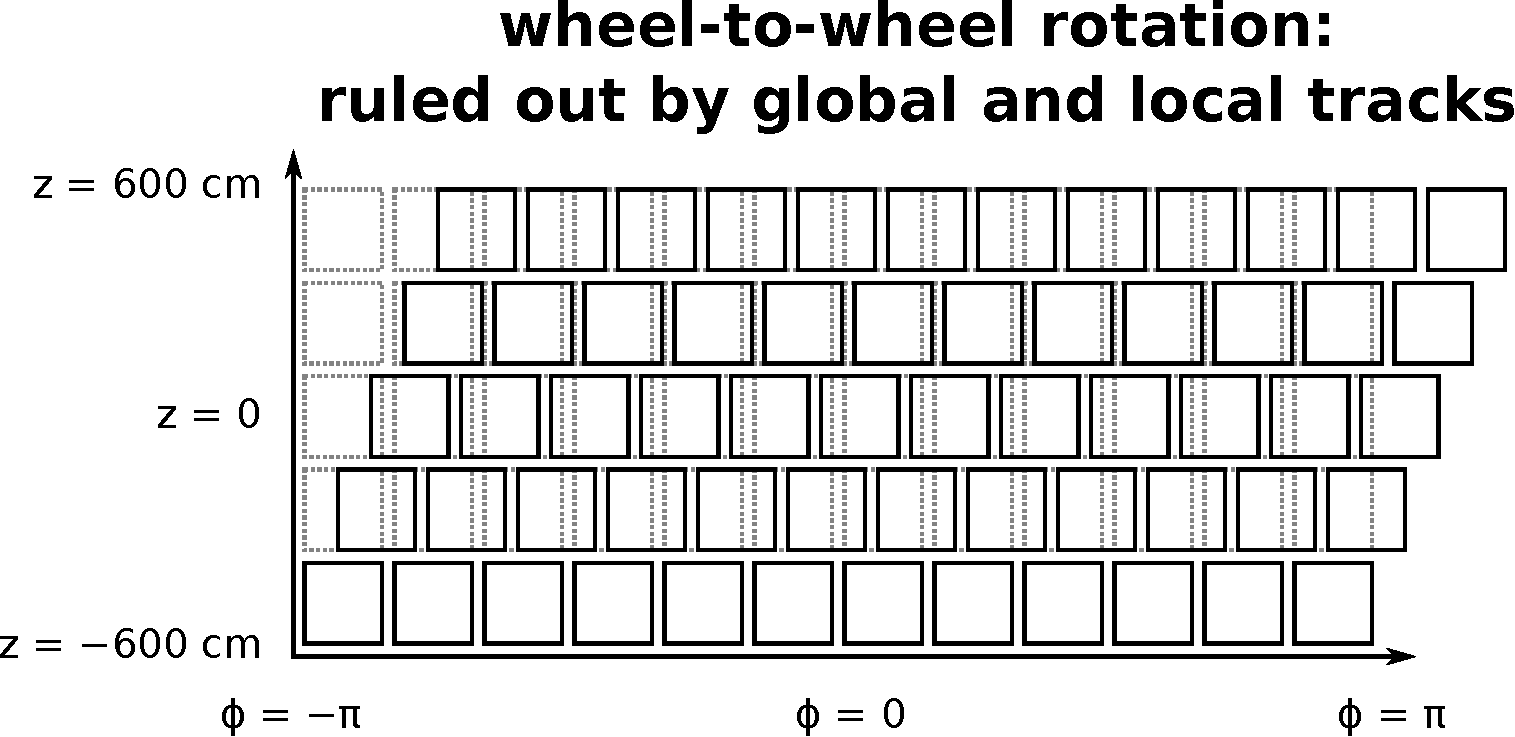
\includegraphics[width=\linewidth]{model1.pdf}
\end{frame}

\begin{frame}
\frametitle{Geometry Models}
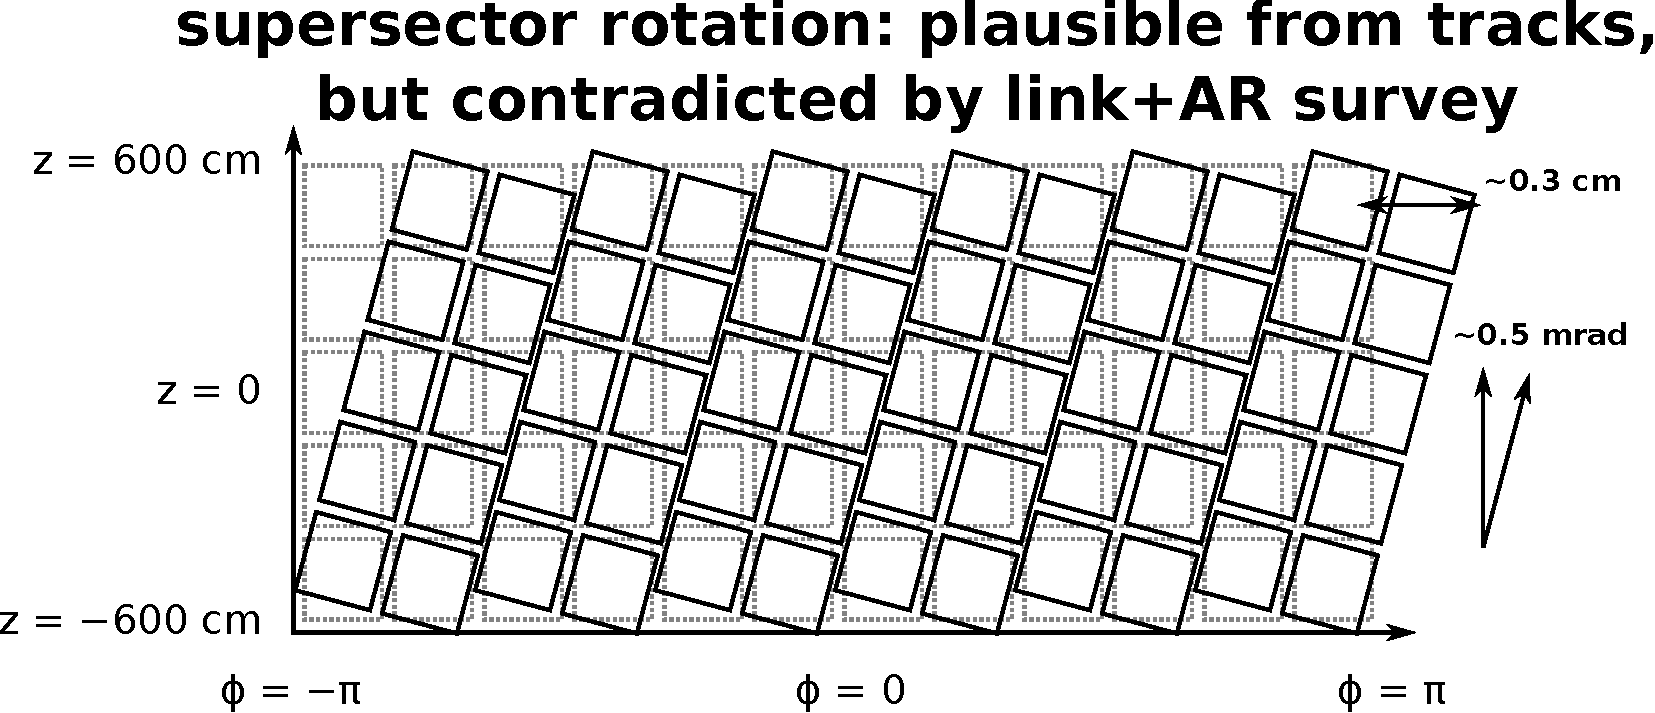
\includegraphics[width=\linewidth]{model2.pdf}
\begin{itemize}
\item It would be interesting to know what the inclinometers and
  transfer lines have to say about this, since they would provide data
  which are independent of the link+AR {\it and} tracks
\item As it stands, it's enough of a problem that link+AR and tracks
  disagree, and that's why we want to investigate more deeply
\end{itemize}
\end{frame}

\begin{frame}
\frametitle{Supersector rotation model: 3D}
\only<1>{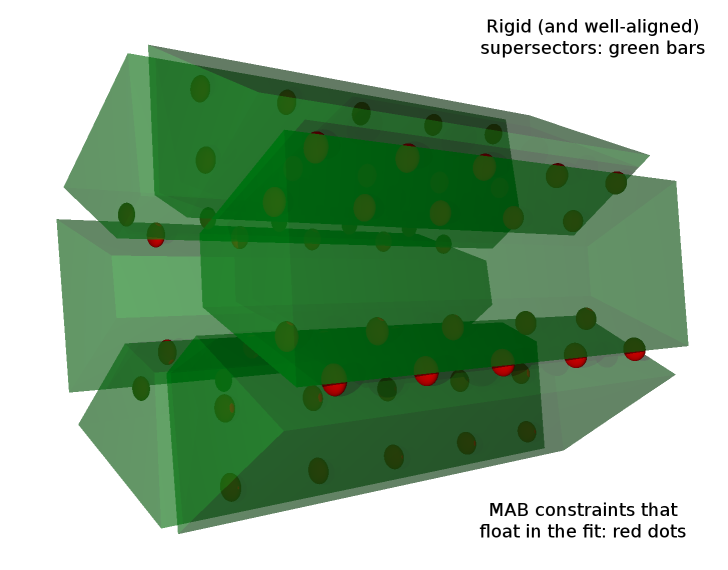
\includegraphics[width=\linewidth]{without_twist.png}}
\only<2>{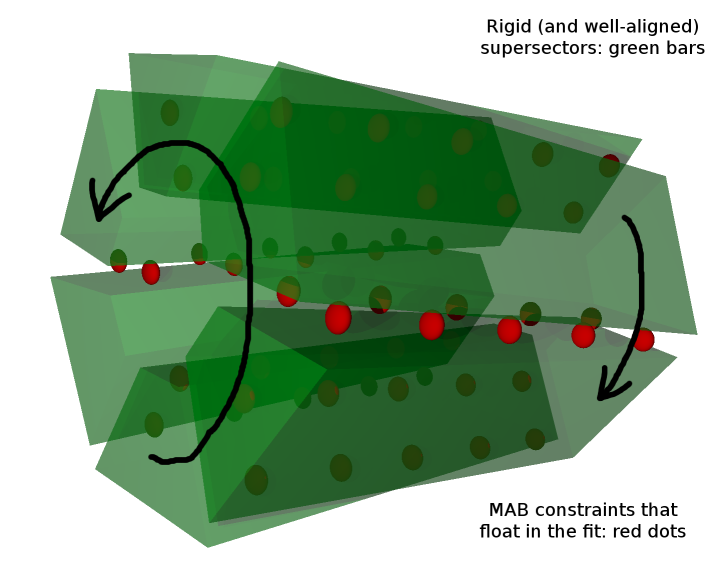
\includegraphics[width=\linewidth]{with_twist.png}}
\only<3>{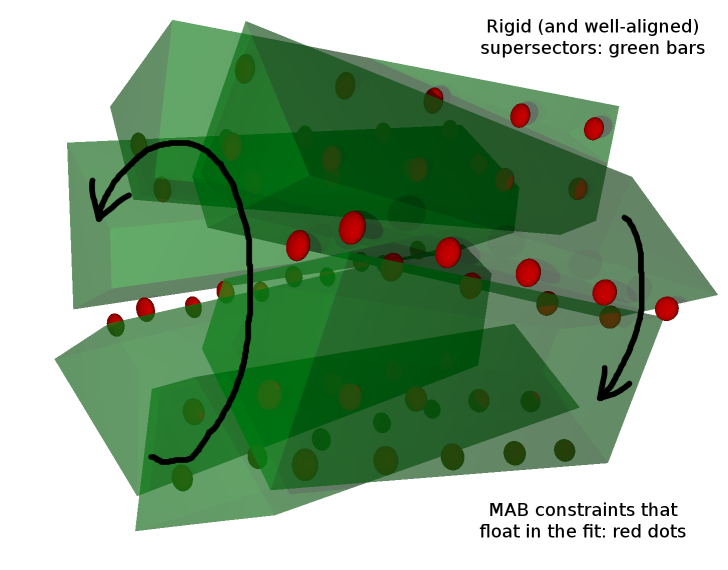
\includegraphics[width=\linewidth]{with_more_twist.png}}
\end{frame}

\begin{frame}
\frametitle{Measurements that could help}
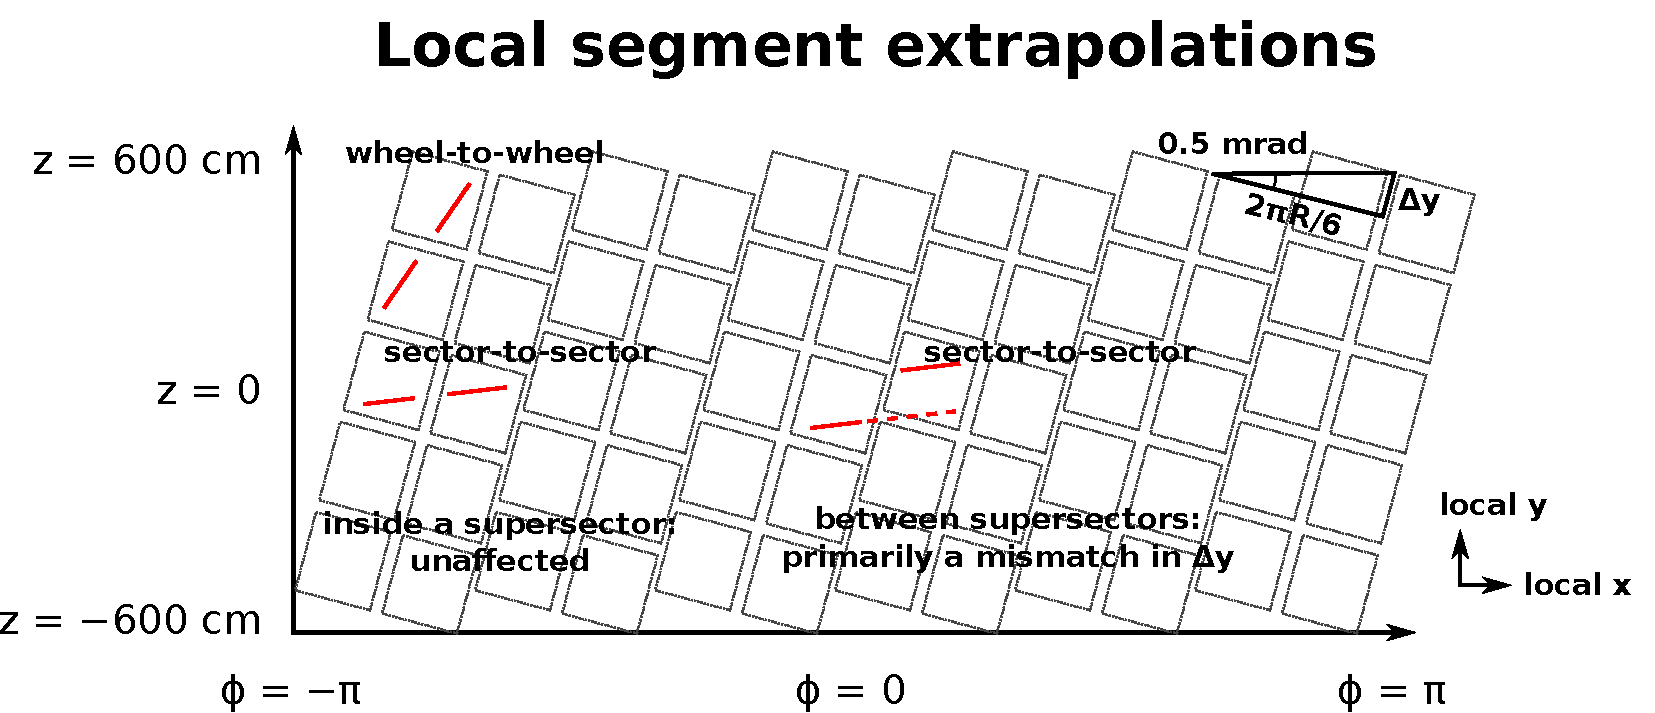
\includegraphics[width=\linewidth]{model2_local.pdf}

\begin{itemize}
\item Should be a constant offset for all wheels, for all 6
  supersector boundaries: $\displaystyle \Delta y = \frac{2\pi R}{6} \, \tan 0.0005
  = 2.6$~mm at $R=5$~m

\item ``Map plot'' style plot of $\Delta y$ vs.\ $\phi$ with a
  multiple of 12 bins (preferably 48 or more) would show
  discontinuities between supersectors and linear slopes between
  them\ldots or not, if the model isn't true
\end{itemize}
\end{frame}

\begin{frame}
\frametitle{Measurements that could help}
\begin{itemize}
\item A ``supersector rotation'' of 0.5~mrad would have the following
  consequences for barrel hardware measurements between neighboring supersectors:

\[ \Delta\phi = 0, \hspace{0.5 cm} \Delta R = \left(Z_{\mbox{\scriptsize pos}}\right) \tan 0.0005, \hspace{0.5 cm} \Delta z = \left(\frac{2\pi R_{\mbox{\scriptsize pos}}}{6}\right) \tan 0.0005 \]

\begin{itemize}
\item $\phi$ and $r\phi$ measurements are {\it completely} insensitive to it
\item the sensitivity of radial measurements are proportional to
  $Z_{\mbox{\scriptsize pos}}$, the distance of the sensor from the
  symmetry plane of CMS
\item the sensitivity of $\Delta z$ measurements are proportional to
  $R_{\mbox{\scriptsize pos}}$, the distance of the sensor from the
  beamline
\end{itemize}

\item I've created a mathematical model to verify the above and to
  search for auxiliary rotations or translations of the supersectors
  that can absorb a ``supersector rotation,'' thus providing for a
  weak mode.  There aren't any: this is a straight-forward measurment.
  If the barrel's inter-supersector measurements are sensitive to
  $\Delta R$ or $\Delta z$ at the level of $\mathcal{O}(\mbox{1 mm})$,
  then it can rule out the effect.
\end{itemize}



\label{numpages}
\end{frame}

%% \section*{First section}
%% \begin{frame}
%% \begin{center}
%% \Huge \textcolor{blue}{First section}
%% \end{center}
%% \end{frame}

\end{document}
